\documentclass{article}
\usepackage{tikz}
\usetikzlibrary{arrows}
\usetikzlibrary{shapes.geometric}
\begin{document}
%\begin{tikzpicture}
%[every node/.style={inner sep=0pt}]
%\node (17) [circle, minimum size=50.0pt, fill=lightgray, line width=1.875pt, draw=black] at (125.0pt, -87.5pt) {\textcolor{black}{\large Q}};
%\node (18) [circle, minimum size=50.0pt, fill=lightgray, line width=1.875pt, draw=black] at (237.5pt, -87.5pt) {\textcolor{black}{\large R}};
%\draw [line width=3.125, ->, color=black] (17) to  [in=210, out=331] (18);
%\draw [line width=3.125, ->, color=black] (18) to  [in=40, out=140] (17);
%\draw [line width=3.125, ->, color=black, loop right] (18) to (18);
%\draw [line width=3.125, ->, color=black, loop left] (17) to (17);
%\node at (181.25pt, -116.875pt) {\textcolor{black}{0.05}};
%\node at (181.25pt, -49.375pt) {\textcolor{black}{0.1}};
%\node at (304.375pt, -87.5pt) {\textcolor{black}{0.9}};
%\node at (55.0pt, -87.5pt) {\textcolor{black}{0.95}};
%\end{tikzpicture}

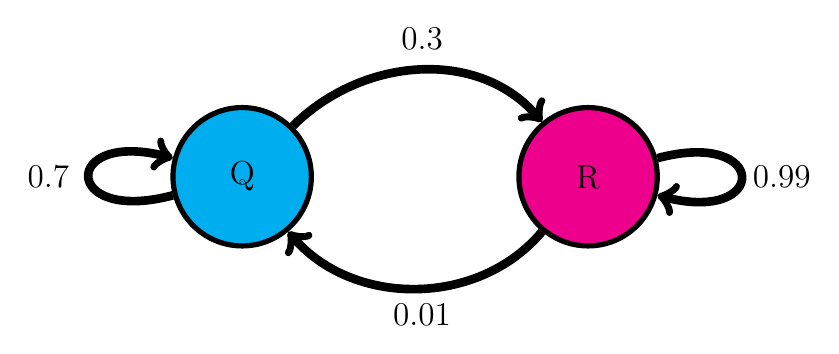
\begin{tikzpicture}
[every node/.style={inner sep=0pt}]
\node (17) [circle, minimum size=50.0pt, fill=cyan, line width=1.875pt, draw=black] at (125.0pt, -90pt) {\textcolor{black}{\large Q}};
\node (18) [circle, minimum size=50.0pt, fill=magenta, line width=1.875pt, draw=black] at (250.0pt, -90pt) {\textcolor{black}{\large R}};
\draw [line width=3.125, ->, color=black] (17) to  [in=130, out=45] (18);
\draw [line width=3.125, ->, color=black] (18) to  [in=310, out=230] (17);
\draw [line width=3.125, ->, color=black, loop right] (18) to (18);
\draw [line width=3.125, ->, color=black, loop left] (17) to (17);
\node at (55pt, -90pt) {\textcolor{black}{\large 0.7}};
\node at (320pt, -90pt) {\textcolor{black}{\large 0.99}};
\node at (190.0pt, -140pt) {\textcolor{black}{\large 0.01}};
\node at (190.0pt, -40pt) {\textcolor{black}{\large 0.3}};
\end{tikzpicture}
\end{document}